\chapter{Departmental Context}

The Coffee Chain ERP system centralizes the management of coffee outlets, sales operations, menu items, and CRM. This integration enhances operational efficiency, reduces manual errors, and provides real-time insights for management, supporting both day-to-day operations and strategic decision-making.

\section*{Departments Covered}

\begin{itemize}
    \item \textbf{Outlet Management:}  
    Maintains critical outlet information such as name, location, manager, and regional manager. Ensures uniform operations and adherence to standards across all outlets. The module allows management to monitor performance and operational compliance regionally and locally.
    
    \item \textbf{Sales Department:}  
    Records all transactions, monitors daily revenue, and produces performance reports. Provides visibility into outlet-specific sales trends, product popularity, and revenue contribution.
    
    \item \textbf{Customer Relationship Management (CRM):}  
    Captures leads, tracks customer interactions, and supports targeted marketing campaigns. Enables management to analyze customer behavior, improve engagement, and optimize sales strategies.
    
    \item \textbf{Menu Management:}  
    Manages coffee and snack items, categories, prices, and optional customization options. Integrated directly with sales for real-time ordering, ensuring consistency and accuracy in product offerings across all outlets.
\end{itemize}

\section*{Operational Workflow}

\begin{enumerate}
    \item Outlets serve as the operational base, with managers overseeing local sales, staff, and inventory.
    \item Menu items are created and updated in the ERP, and automatically synced with the sales module to ensure accurate pricing and availability.
    \item Sales transactions are captured per outlet and feed into automated performance dashboards, providing insight into revenue, popular products, and sales trends.
    \item CRM collects customer data and tracks engagement, supporting lead conversion, loyalty efforts, and targeted marketing campaigns.
\end{enumerate}

\section*{QMS and PDCA Integration}

The ERP system incorporates Quality Management System (QMS) principles using the PDCA (Plan-Do-Check-Act) methodology:

\begin{itemize}
    \item \textbf{Plan:} Design workflows for outlets, sales, menu, and CRM to ensure smooth and standardized operations.
    \item \textbf{Do:} Implement the ERP system with integrated modules and train staff for consistent usage.
    \item \textbf{Check:} Monitor key performance indicators (KPIs) such as revenue per outlet, product sales, lead conversion rates, and customer engagement.
    \item \textbf{Act:} Refine operational procedures, update ERP configurations, and implement corrective measures based on performance analysis.
\end{itemize}


\textbf{Department Interaction Diagram:}  


\begin{figure}[H]
\centering
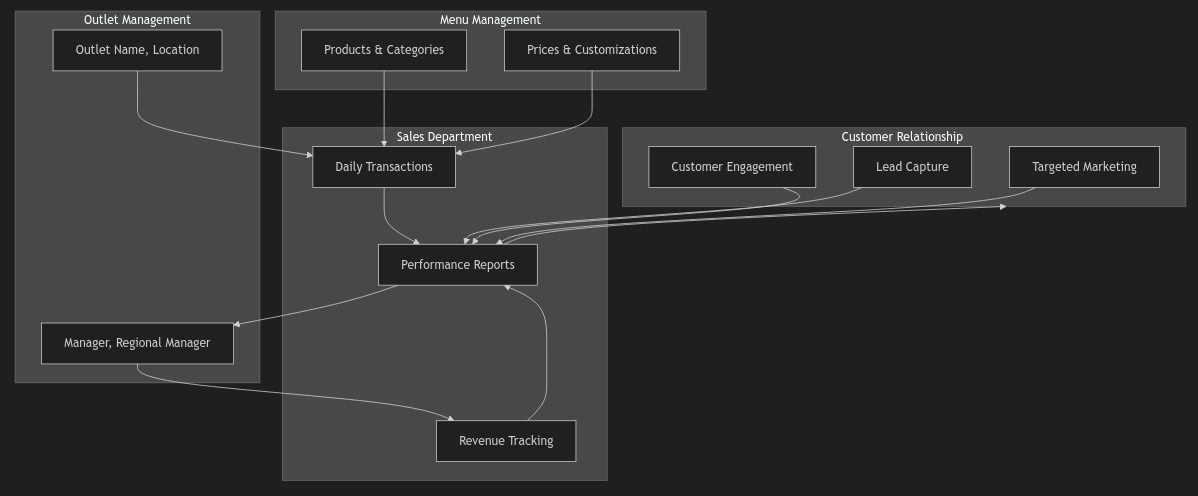
\includegraphics[width=0.9\textwidth,height=0.5\textheight,keepaspectratio]{diagrams/department.png}
\caption{Department Interaction Diagram of Coffee Chain ERP}
\end{figure}

\section*{Insights}

\begin{itemize}
    \item Centralizing departmental operations ensures consistency and reduces redundancies.
    \item Automated data flow from menu to sales and CRM improves accuracy and responsiveness.
    \item PDCA integration allows continuous improvement, ensuring the ERP evolves to meet operational needs.
    \item Management gains comprehensive oversight across outlets, enabling data-driven strategic decisions.
\end{itemize}
